% latex template for a report
% written by Michael McClintock

\RequirePackage[l2tabu, orthodox]{nag} % warnings for obsolete stuff
\documentclass[12pt,a4paper]{article}  % article class

% font setup
\usepackage{ifluatex}
\ifluatex
    \usepackage[no-math]{fontspec} % keep standard math
    \setmainfont[Ligatures=TeX]{Linux Libertine}
    \setsansfont[Ligatures=TeX]{Linux Biolinum}
    \setmonofont[Ligatures=TeX]{Inconsolata}
\else
    \usepackage[T1]{fontenc}
    \usepackage{inconsolata}
\fi
\usepackage{microtype}

% useful packages
\usepackage[svgnames]{xcolor}          % color commands
\usepackage{graphicx}                  % including graphics (use eps)
\usepackage[margin=20mm]{geometry}     % set margins
\usepackage{amsmath,amssymb,cancel,bm} % math \bm for bold math
\usepackage[hidelinks]{hyperref}       % clickable links
\usepackage{url}                       % format urls
\usepackage{cleveref}                  % convenient refrencing use \Cref
\usepackage{paralist}                  % compact itemize/enumerate
\usepackage[hang, small, bf, margin=20pt]{caption} % captions for figures
\usepackage{setspace}%\onehalfspacing               % 1.5 line spacing
\setlength{\parindent}{0cm}\usepackage{parskip}    % paragraph skip
\usepackage[                                   % SI units
    load-configurations=abbreviations,         % unit abrev.
    separate-uncertainty=true,                 % plus minus in uncertainty
    inter-unit-product=\ensuremath{{}\cdot{}}, % dot between units
    per-mode=symbol-or-fraction                % per style
]{siunitx}
\usepackage[nottoc,numbib]{tocbibind} % refs in toc

\begin{document}

% title page
\begin{titlepage}
\begin{center}
\textsc{\LARGE PHYS3900 Final Project}\\[1cm]
{\LARGE Content Generation for Smartphone Based Physics Learning}\\[2cm]
\begin{minipage}[t]{0.6\columnwidth} \large
\begin{description}
\itemsep2mm
\small
\item [\emph{Author:}] Michael McClintock (41757129)
\item [\emph{Partner:}] Alex van Nunen
\item [\emph{Date:}] October 8, 2012
\item [\emph{Email:}] michael.mcclintock@uqconnect.edu.au
\item [\emph{Supervisors:}] -
\end{description}
\end{minipage}
\vfill
\end{center}
\end{titlepage}

% abstract
\begin{abstract}
Ab.
\end{abstract}
\thispagestyle{empty}
\newpage

% table of contents
\tableofcontents
\thispagestyle{empty}
\newpage
\setcounter{page}{1}

% sections
\section{Introduction and Background}

% It is no secret that smartphones, tablets and other portable
% multimedia devices are on the rise. As reported in February 2012,
% 487.7 million smartphones were shipped worldwide 2011.  This figure,
% up 63\% from 2010, also meant that smarthphone sales have overtaken
% the sale of personal computers \cite{canalys}. 

% There are a number of factors that make smartphone based learning
% (often referred to as ubiquitous learning or just ``u-learning") an
% effective, if not inevitable, complement to the more traditional
% methods of course and content delivery. These factors include the
% widespread smartphone reliance of university students and staff, high
% convenience, powerful multimedia capabilities and good wireless and
% internet connectivity \cite{worry}.

% While many universities have developed campus-wide tools for
% smartphones. The use of u-learning solutions tailor-made for specific
% courses or subject areas is not widely accepted \cite{procsmart}.
% One reason is the lack of mature technology for content delivery that
% addresses technical issues such as platform independence. Another is the
% lack of examples and trials related to the design of content for
% u-learning systems.

% This project has two separate goals. The first is to find a simple
% solution that allows the delivery of u-learning content to smartphones
% and tablets. The second and more important goal is to produce and test
% some u-learning material for first year physics students.

% While subject specific u-learning material is a relatively new concept
% there is a great deal of research into what makes good ``e-learning"
% material where e-learning refers to the use of computers and internet
% in learning. Many of the generally accepted approaches to e-learning
% may be equally effective when transferred to a smartphone based
% system.

% \section*{Significance of Research and Expected Outcomes}

% Any method or aid that helps students absorb and understand a topic at
% a fundamental level is valuable to instructors. Finding this type of
% tool for physics is even more significant because the ideas and
% concepts of physics are generally more abstract and fundamental
% compared to other subject areas. 

% Designing, implementing and testing a u-learning system for a small
% part of a first year physics course allows for evaluation of the
% effectiveness of smartphone based systems. Following this project
% instructors should have some evidence of the advantages or
% disadvantages of u-learning systems for first year physics. As well as
% some ideas about how to create their own systems.

\section{Methodology and Design}

\subsection{Content format}

In order to address the project goals we started by looking at the content
format. What is an effective way to author content for a physics app and for
physics in general? Below are some characteristics of the content format which
we thought were important.

\begin{itemize}
\item First the format should be simple. The generation of quality physics content is what the author should be focusing on. The format shouldn't get in the way. It should be simple enough that anyone can write content for the apps.
\item The format should be a well established standard with tested tools for conversion to other formats.
\item It should be easy to insert text, math equations, images, videos links and references.
\end{itemize}

Using the above charecteristics the format we decided to use for this project was Markdown QUOTE!. Perhaps the best way to describe Markdown is by example. \Cref{fig:md} shows some markdown text along with the final output on a mobile device. The example shows a heading, an image, text and a math equation (using tex notation).

\begin{figure}[htb]
\rule[0.5ex]{1\columnwidth}{1pt}
\footnotesize
\begin{verbatim}
# Buoyancy

![ ](/static/Fluid3.png)

Take the block of water inside the bucket on the left hand side. This
block of water is being upheld by the pressure in the liquid
underneath the block of water, while being pressed down by the force
of gravity.  Since this block of water is stationary, that means that
the force of gravity equals the force of buoyancy. So at this point:

$F_{gravity}=F_{buoyant}=m_f g$
\end{verbatim}
\rule[0.5ex]{1\columnwidth}{1pt}
\\[2mm]
\centering
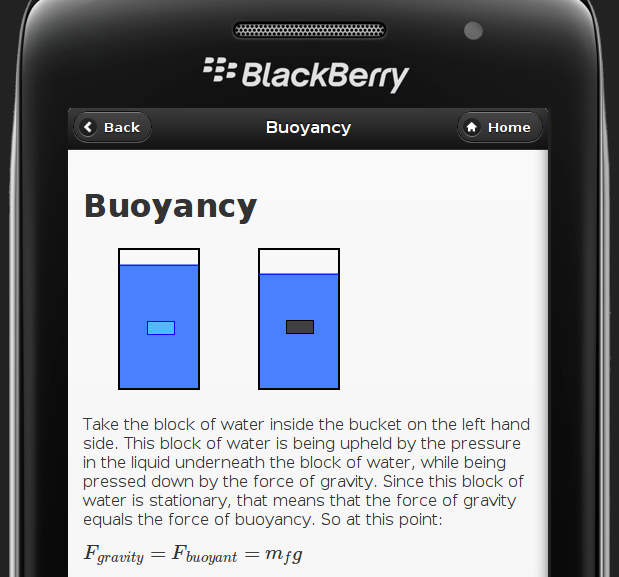
\includegraphics[width=0.45\textwidth]{buoyancy.png}
\caption{Markdown input (top), Final output (bottom)}
\label{fig:md}
\end{figure}


\subsection{s}





































% Again when it comes to designing the solution there are two separate
% aspects. The first is the method of delivering the content and the
% second is the design of the content itself. While the second aspect is
% the main focus of the project it cannot be tested without an effective
% solution to the problem of content delivery.


% \subsubsection*{Content Delivery}

% Web 2.0 technologies such as blogs, wikis and interactive websites
% have changed the face of online interaction and collaboration
% \cite{procsmart}. These online applications are becoming good enough
% that at times it's hard to know you're not running a native application
% on your PC. Also it is worth noting that web technologies (HTML, CSS
% and javascript) are open-source, cross-platform, widespread and mature. 

% The major problem of delivering content effectively to the large
% number of smartphone and tablet like devices is dealing with their
% differences.  To develop a native application for Android users, the
% developer must be proficient with java and understand the Android
% specific libraries. A similar but conflicting approach is needed for
% iOS devices where one must understand Objective-C programming and the
% Apple specific toolkits. This all becomes very overwhelming when the
% goal is to achieve a simple content delivery system. 

% Luckily web browsers exist on all devices that comply to standard web
% technologies. This makes it possible to design u-learning content and
% then deliver it to the multitude of device in a consistent
% maintainable format. One project that aims to simplify this process is
% called PhoneGap \cite{phonegap}. To achieve simple content delivery
% this project aims to follow the approach of developing u-learning
% material using web technologies that are deliverable to a number of
% devices using technologies such as PhoneGap.

% \subsubsection*{U-Learning Physics Content}

% The content itself will be tailored to first year physics students at
% the University of Queensland. More specifically this project will be
% targeting the Fluids component of PHYS1171. The material will focus
% on the topics of pressure/depth, buoyancy and the fluid dynamics of
% non-viscous fluids. Both Alex and I will choose a topic to
% construct material for. The proposed method is as follows

% \begin{itemize}
%   \item Brainstorm available methods and construct a concept map
%   \item Select appropriate material from available sources
%   \item Prototype the material and deliver to devices
%   \item Develop test for students and structure for feedback
%   \item Analyse feedback
%   \item Write report with results and future recommendations/changes
% \end{itemize}

% The approach to designing content will be to look at effective content
% in e-learning systems aimed specifically at physics. A good example is
% the design of effective physics videos \cite{vid}. Videos and
% animation based content isn't the only way to keep users interested.
% Simple things like the format and style of accompanying text and
% graphics matter. When designing the solution we will look for
% resources and examples of effective content layout and styling on
% mobile devices. If time permits the possibility of adding interactive
% components like the ability for users to leave comments will be looked
% at.

% \section*{Timeline}

% \begin{itemize}
% \item Week 1-3. Familiarisation with topic. Produce Written proposal.  
% \item Week 3-4. Research into physics content best
%   practices.  Develop the structure of the content to be presented
% \item Week 4-5. Develop preliminary content using web technologies
% \item Week 5-6. Find/implement a simple method for delivering the
%   preliminary content to physical devices 
% \item Week 7-8. Refine material and prepare for trial on students 
% \item week 8-9. Test system on students and collect feedback 
% \item week 9-10. Analyse results and prepare report
% \end{itemize}

\bibliographystyle{ieeetr}
\bibliography{refs}

\end{document}
